\chapter{Compilation}
\label{chp:compilation}
The following chapter presents the considerations and translation schemas used in the process of translating \rooplpp to the reversible low-level machine language \textsc{Pisa}. As \rooplpp is an extension of \textsc{Roopl}, many techniques are carried directly over, and have as such been left out.

Before presenting the \rooplpp compiler, a brief overview of the memory layout and modeling of the \textsc{Roopl} compiler, which the \rooplpp compiler is a continuation of, is provided. 

\section{The \textsc{Roopl} to \textsc{Pisa} Compiler}
\label{sec:roopl-to-pisa-compiler}
\citeauthor{th:roopl} presented a proof-of-concept compiler along with the design for \textsc{Roopl}. The compiler translates well-typed \textsc{Roopl} programs into the reversible machine language \textsc{Pisa} in~\cite{th:roopl}. The \textsc{Roopl} compiler (\textsc{RooplC}) is written in \textsc{Haskell} and hosted at \url{https://github.com/TueHaulund/ROOPLC}.

\begin{figure}[ht]
    \centering
    \begin{tikzpicture}
        \fill[fill = grey] (6, 0) rectangle (8, 3) node[midway] {Stack};
        \draw (6, 0) -- (12, 0);
        \draw (6, 3) -- (12, 3);
        \draw (12, 0) -- (12, 3);
        \draw[dashed] (8, 0) -- (8, 3);
    
        \filldraw[fill = grey, draw = black] (0, 0) rectangle (2.5, 3) node[midway] {Static Data};
        \filldraw[fill = darkgrey, draw = black] (2.5, 0) rectangle (6, 3) node[midway] {Program};
        
        \node at (10, 2.5) {(unused memory)};
        \node at (0, -.3) {$0$};
        \node at (6, -.3) {$p$};
        \node at (8, -.3) {$sp$};
        \node at (12, -.3) {$2^{31} - 1$};
        \node at (6, -1) {$\longleftarrow$ Address Space $\longrightarrow$};
        \draw[arrow, dashed] (8, 1.5) -- (10, 1.5);
        \node at (8.9, 1.2) {\scriptsize{\textit{stack grows}}};
    \end{tikzpicture}
    \caption{Memory layout of a \textsc{Roopl} program, originally from~\cite{th:roopl}}
    \label{fig:roopl-memory-layout}
\end{figure}

Figure~\ref{fig:roopl-memory-layout} shows the memory layout of a compiled \textsc{Roopl} program. The layout consists of a static storage segment, the program segment and the stack. 

\begin{figure}[ht]
    \centering
    \begin{subfigure}[t]{.32\textwidth}
        \vskip 0pt
        \centering
        \begin{tikzpicture}
            \draw[dashed] (0, 1.5) -- (0, 2);
            \draw[dashed] (3, 1.5) -- (3, 2);
            \filldraw[fill = grey, draw = black] (0, 1) rectangle (3, 1.5) node[midway] {addr(vtable)};
            \filldraw[fill = darkgrey, draw = black] (0, .5) rectangle (3, 1) node[midway] {x};
            \filldraw[fill = grey, draw = black] (0, 0) rectangle (3, .5) node[midway] {y};
            \draw[dashed] (0, 0) -- (0, -.5);

            \draw[dashed] (3, 0) -- (3, -.5);
    
            \node at (-.3, 1.25) {\texttt{+}$0$};
            \node at (-.3, .75) {\texttt{+}$1$};
            \node at (-.3, .25) {\texttt{+}$2$};
            \draw[->] (3.5, 1.25) -- (3.1, 1.25);
            \node[rotate = 270] at (3.7, 1.25) {$r_{shape}$};
            
            \node at (1.5, 2.5) {\textbf{Shape}};
        \end{tikzpicture}
    \end{subfigure}
    \begin{subfigure}[t]{.32\textwidth}
        \vskip 0pt
        \centering
        \begin{tikzpicture}
            \draw[dashed] (0, 1.5) -- (0, 2);
            \draw[dashed] (3, 1.5) -- (3, 2);
            \filldraw[fill = grey, draw = black] (0, 1) rectangle (3, 1.5) node[midway] {addr(vtable)};
            \filldraw[fill = darkgrey, draw = black] (0, .5) rectangle (3, 1) node[midway] {x};
            \filldraw[fill = grey, draw = black] (0, 0) rectangle (3, .5) node[midway] {y};
            \filldraw[fill = darkgrey, draw = black] (0, -.5) rectangle (3, 0) node[midway] {radius};
            \draw[dashed] (0, -.5) -- (0, -1);
            \draw[dashed] (3, -.5) -- (3, -1);
    
            \node at (-.3, 1.25) {\texttt{+}$0$};
            \node at (-.3, .75) {\texttt{+}$1$};
            \node at (-.3, .25) {\texttt{+}$2$};
            \node at (-.3, -.25) {\texttt{+}$3$};
            \draw[->] (3.5, 1.25) -- (3.1, 1.25);
            \node[rotate = 270] at (3.7, 1.25) {$r_{circ}$};
            
            \node at (1.5, 2.5) {\textbf{Circle}};
        \end{tikzpicture}
    \end{subfigure}
    \begin{subfigure}[t]{.32\textwidth}
        \vskip 0pt
        \centering
        \begin{tikzpicture}
            \draw[dashed] (0, 1.5) -- (0, 2);
            \draw[dashed] (3, 1.5) -- (3, 2);
            \filldraw[fill = grey, draw = black] (0, 1) rectangle (3, 1.5) node[midway] {addr(vtable)};
            \filldraw[fill = darkgrey, draw = black] (0, .5) rectangle (3, 1) node[midway] {x};
            \filldraw[fill = grey, draw = black] (0, 0) rectangle (3, .5) node[midway] {y};
            \filldraw[fill = darkgrey, draw = black] (0, -.5) rectangle (3, 0) node[midway] {a};
            \filldraw[fill = grey, draw = black] (0, -1) rectangle (3, -.5) node[midway] {b};
            \draw[dashed] (0, -1) -- (0, -1.5);
            \draw[dashed] (3, -1) -- (3, -1.5);
    
            \node at (-.3, 1.25) {\texttt{+}$0$};
            \node at (-.3, .75) {\texttt{+}$1$};
            \node at (-.3, .25) {\texttt{+}$2$};
            \node at (-.3, -.25) {\texttt{+}$3$};
            \node at (-.3, -.75) {\texttt{+}$4$};
            \draw[->] (3.5, 1.25) -- (3.1, 1.25);
            \node[rotate = 270] at (3.7, 1.25) {$r_{rect}$};
            
            \node at (1.5, 2.5) {\textbf{Rectangle}};
        \end{tikzpicture}
    \end{subfigure}
    
    \caption[Illustration of object memory layout]{Illustration of prefixing in the memory layout of 3 \textsc{Roopl} objects, originally from~\cite{th:roopl}}
    \label{fig:roopl-object-layout}
\end{figure}

The object model is simple and only features one additional word for storing the address of the virtual table for the object class. Figure~\ref{fig:roopl-object-layout} shows the prefixing for three simple classes modeling geometric shapes.


\section{\rooplpp Memory Layout}
\label{sec:rooplpp-memory-layout}
\rooplpp builds upon the memory layout of its predecessor  with dynamic memory management. The reversible Buddy Memory heap layout presented in section~\ref{subsec:buddy-memory} is utilized in \rooplpp as it is an interesting layout, addressing a number of disadvantages found in other considered layouts, naturally translates into a reversible setting with one simple restriction (i.e only blocks which are heads of their respectable free lists are allocatable) and since its only drawback is dismissible in most real world scenarios.

\begin{figure}[ht]
    \centering
    \begin{tikzpicture}
        \fill[fill = grey] (0, 0) rectangle (2.5, 3) node[midway] {Static Data};
        \fill[fill = darkgrey] (2.5, 0) rectangle (5, 3) node[midway] {Program};
        \fill[fill = grey] (5, 0) rectangle (7, 3) node[midway] {Free lists};
        \fill[fill = grey] (7, 0) rectangle (8.5, 3) node[midway] {Heap};
        \fill[fill = grey] (12.5, 0) rectangle (14, 3) node[midway] {Stack}; 
        
        \draw (0, 0) -- (15, 0);
        \draw (0, 3) -- (15, 3);
        \draw (0, 0) -- (0, 3);
        \draw (15, 0) -- (15, 3);
        \draw (2.5, 0) -- (2.5, 3);
        \draw (5, 0) -- (5, 3); 
        \draw (7, 0) -- (7, 3);
        \draw (14, 0) -- (14, 3); 
        \draw[dashed] (8.5, 0) -- (8.5, 3); 
        \draw[dashed] (12.5, 0) -- (12.5, 3);   
    
        \node at (10.5, 2.5) {(unused memory)};
        \node at (0, -.3) {$0$};
        \node at (5, -.3) {$flp$};
        \node at (7, -.3) {$hp$};
        \node at (14, -.3) {$p$};
        \node at (12.5, -.3) {$sp$};
        \node at (15, -.3) {$2^{31} - 1$};
        \node at (7.5, -1) {$\longleftarrow$ Address Space $\longrightarrow$};

        \draw[arrow, dashed] (8.5, 1.5) -- (10.1, 1.5);
        \node at (9.4, 1.2) {\scriptsize{\textit{heap grows}}};

        \draw[arrow, dashed] (12.5, 1.5) -- (10.9, 1.5); 
        \node at (11.6, 1.2) {\scriptsize{\textit{stack grows}}};
    \end{tikzpicture}
    \caption{Memory layout of a \rooplpp program}
    \label{fig:memory-layout}
\end{figure}

Figure~\ref{fig:memory-layout} shows the full layout of a \rooplpp program stored in memory.

\begin{itemize}
    \item As with \textsc{Roopl}, the static storage segment contains load-time labelled \inst{data} pseudo-instructions, initialized with virtual function tables and other static data needed by the translated program.

    \item The program segment is stored right after the static storage and contains the translated \rooplpp program instructions.

    \item The free lists maintained by the Buddy Memory heap layout is placed right after the program segment, with the \textit{free list pointer} $flp$ pointing at the first free list. The free lists are simply the address pointing to the first block of its respective size. The free lists are stored such that the free list at address $flp + i$ corresponds to the free list of size $2^{i+1}$.   

    \item The heap begins directly following the free lists. Its beginning is marked by the \textit{heap pointer} $(hp)$. 

    \item Unlike in \textsc{Roopl}, where the stack grows upwards, the \rooplpp stack grows downwards and begins at address $p$. The stack remains a LIFO structure, analogously to \textsc{Roopl}.
\end{itemize}

As mentioned in the previous chapter, we assume an underlying reversible operating system providing us with additional memory when needed. With no real way of simulating this, the \rooplpp compiler places the stack at a fixed address $p$ and sets one free block in the largest $2^n$ free list initially. The number of free lists and the address $p$ is configurable in the source code, but defaults to $10$ free lists, meaning initially one block of size $1024$ is available and the stack is placed at address $1024$ words after the heap.

In traditional compilers, the heap pointer usually points to the end of the heap. For reasons stated above, we never grow the heap as we start with a heap of fixed size. As such, the heap pointer simply points to the beginning of the heap.

The heap can simply be expanded by adding another block of the largest possible size and storing the address of the respective free list.

In the following sections of this chapter, we will present various translation techniques. In these translations, we will make use of a number of \textsc{Pisa} pseudo-instructions to subtract integer values from registers and pushing/popping to the program stack. The pseudo-instructions are shown in figure~\ref{fig:pseudo-instructions} and are modified from~\cite{th:roopl}, as the direction of the program stack is flipped in \rooplpp.

\begin{figure}[ht]
    \centering
    \begin{alignat*}{2}
        \inst{subi}\quad r\quad i \qquad &\overset{\textbf{def}}{\scalebox{1.8}{=}} \qquad&&\ \inst{addi}\quad r\quad -i\\[1.6ex]
        \inst{push}\quad r \qquad &\overset{\textbf{def}}{\scalebox{1.8}{=}} \qquad&&\Big[\inst{exch}\quad r\quad r_{sp}\ , \quad \inst{subi}\quad r_{sp}\quad 1\Big]\\[1.6ex]
        \inst{pop}\quad r \qquad &\overset{\textbf{def}}{\scalebox{1.8}{=}} \qquad&&\Big[\inst{addi}\quad r_{sp}\quad 1\ , \quad \inst{exch}\quad r\quad r_{sp}\Big]
    \end{alignat*}
    \caption{Definition of pseudoinstructions \inst{subi}, \inst{push} and \inst{pop}, modified from~\cite{th:roopl}}
    \label{fig:pseudo-instructions}
\end{figure}


\section{Inherited \textsc{Roopl} features}
\label{sec:inherited-features}
As mentioned, a number of features from \textsc{Roopl} carries over to \rooplpp.

The dynamic dispatching mechanism presented in~\cite{th:roopl} is inherited. As such, the invocation of a method implementation is based on the type of the object at run time. Virtual function tables are still the implementation strategy used in the dynamic dispatching implementation.

Evaluation of expressions and control flow remains unchanged. 

For completeness, object blocks are included and still stack allocated as their life time is limited to the scope of their block and the dynamic allocation process is quite expensive in terms of register pressure and number of instructions compared to the stack allocated method implemented in the \textsc{Roopl} compiler.


\section{Program Structure}
\label{sec:program-structure}
The program structure of a translated \rooplpp is analogous to the program structure of a \textsc{Roopl} program with the addition of free lists and heap initialization. The full structure is shown in figure~\ref{fig:pisa-program-layout}. 

\begin{figure}[ht]
    \centering
    \resizebox{.8\linewidth}{!}{
        \begin{minipage}{\linewidth}
            \begin{alignat*}{6}
                &\textbf{(1)}\quad&& &&\cdots\cdots && && &&\text{; Static data declarations}\\
                &\textbf{(2)}\quad&& &&\cdots\cdots && && &&\text{; Code for program class methods}\\
                &\textbf{(3)}\quad&&start\ \texttt{:}\quad&&\inst{start}\quad&& && &&\text{; Program starting point}\\
                &\textbf{(4)}\quad&& &&\inst{addi}\quad &&r_{flps}\quad &&p&&\text{; Initialize free lists pointer}\\
                &\textbf{(5)}\quad&& &&\inst{xor}\quad &&r_{hp}\quad &&r_{flps}\qquad &&\text{; Initialize heap pointer}\\
                &\textbf{(6)}\quad&& &&\inst{addi}\quad &&r_{hp}\quad &&size_{fls}&&\text{; Initialize heap pointer}\\
                &\textbf{(7)}\quad&& &&\inst{xor}\quad &&r_{b}\quad &&r_{hp}\qquad &&\text{; Store address of initial free memory block in $r_b$}\\
                &\textbf{(8)}\quad&& &&\inst{ADDI}\quad &&r_{flps}\quad &&size_{fls}\quad &&\text{; Index to end of free lists}\\
                &\textbf{(9)}\quad&& &&\inst{SUBI}\quad &&r_{flps}\quad && 1\quad &&\text{; Index to last element of free lists}\\
                &\textbf{(10)}\quad&& &&\inst{EXCH}\quad &&rb\quad &&r_{flps}\quad &&\text{; Store address of first block in last element of free lists}\\
                &\textbf{(11)}\quad&& &&\inst{ADDI}\quad &&r_{flps}\quad && 1\quad &&\text{; Index to end of free lists}\\
                &\textbf{(12)}\quad&& &&\inst{SUBI}\quad &&r_{flps}\quad &&s\quad &&\text{; Index to beginning of free lists}   \\
                &\textbf{(13)}\quad&& &&\inst{xor}\quad &&r_{sp}\quad &&r_{hp} &&\text{; Initialize stack pointer}\\
                &\textbf{(14)}\quad&& &&\inst{addi}\quad &&r_{sp}\quad &&offset_{stack}\ &&\text{; Initialize stack pointer}\\
                &\textbf{(15)}\quad&& &&\inst{subi}\quad &&r_{sp}\quad &&size_m\qquad &&\text{; Allocate space for main object}\\
                &\textbf{(16)}\quad&& &&\inst{xor}\quad &&r_m\quad &&r_{sp}\qquad &&\text{; Store address of main object in $r_m$}\\
                &\textbf{(17)}\quad&& &&\inst{xori}\quad &&r_v\quad &&label_{vt}\qquad &&\text{; Store address of vtable in $r_v$}\\
                &\textbf{(18)}\quad&& &&\inst{push}\quad &&r_v\quad && &&\text{; Push address of vtable onto stack}\\
                &\textbf{(19)}\quad&& &&\inst{push}\quad &&r_m\quad && &&\text{; Push '\textit{this}' onto stack}\\
                &\textbf{(20)}\quad&& &&\inst{bra}\quad &&label_m \span\omit\span \qquad&&\text{; Call main procedure}\\
                &\textbf{(21)}\quad&& &&\inst{pop}\quad &&r_m\quad && &&\text{; Pop '\textit{this}' from stack}\\
                &\textbf{(22)}\quad&& &&\inst{pop}\quad &&r_v\quad && &&\text{; Pop vtable address into $r_v$}\\
                &\textbf{(23)}\quad&& &&\inst{xori}\quad &&r_v\quad &&label_{vt}\qquad &&\text{; Clear $r_v$}\\
                &\textbf{(24)}\quad&& &&\inst{xor}\quad &&r_m\quad &&r_{sp}\qquad &&\text{; Clear $r_m$}\\
                &\textbf{(25)}\quad&& &&\inst{addi}\quad &&r_{sp}\quad &&size_m\qquad &&\text{; Deallocate space of main object}\\
                &\textbf{(26)}\quad&& &&\inst{subi}\quad &&r_{sp}\quad &&offset_{stack} &&\text{; Clear stack pointer}\\
                &\textbf{(27)}\quad&& &&\inst{xor}\quad &&r_{sp}\quad &&r_{hp} &&\text{; Clear stack pointer}\\
                % &\textbf{(28)}\quad&& &&\inst{subi}\quad &&r_{hp}\quad &&size_{fls} &&\text{; Clear heap pointer}\\
                % &\textbf{(29)}\quad&& &&\inst{xor}\quad &&r_{hp}\quad &&r_{flsp} &&\text{; Clear heap pointer}\\
                % &\textbf{(30)}\quad&& &&\inst{subi}\quad &&r_{flps}\quad &&p &&\text{; Clear free lists pointer}\\
                &\textbf{(28)}\quad&&finish\ \texttt{:}\quad&&\inst{finish}\quad && && &&\text{; Program exit point}
            \end{alignat*}
        \end{minipage}
    }
    \caption{Overall layout of a translated \rooplpp program}
    \label{fig:pisa-program-layout}
\end{figure}

The following \textsc{Pisa} code block initializes the free lists pointer, the heap pointer, the stack pointer, allocates the main object on the stack, calls the main method, deallocates the main object and finally clears the free lists, heap and stack pointers.

The free lists pointer is initialized by adding the base address, which varies with the size of the translated program, to the register $r_{flps}$. In figure~\ref{fig:pisa-program-layout} the base address is denoted by $p$.

The heap pointer is initialized directly after the free lists pointer by adding the size of the free lists. One free list is the size of one word and the full size of the free lists is configured in the source code (defaulted to 10, as described earlier).

Once the heap pointer and free lists pointer is initialized, the initial block of free memory is placed in the largest free lists by indexing to said list, by adding the length of the list of free lists, subtracting 1, writing the address of the first block (which is the same address as the heap pointer, which points to the beginning of the heap) to the last free list and then resetting the free lists pointer to point to the first list again, afterwards.

The stack pointer is initialized simply by adding the stack offset to the heap pointer register $r_{hp}$. The stack offset is configured in the source code and defaults to $1024$, as described earlier in this chapter. As such, the heap and the stack each have $1024$ words of space to utilize. Once the stack pointer has been initialized, the main object is allocated on the stack and the main method called, analogously to the \textsc{Roopl} program structure.

When the program terminates and the main method returns, the main object is popped from the stack and deallocated and the stack pointer is cleared. The heap and free list pointer not intentionally not cleared to simulate future program simulation using these pointers. The contents of the free lists and whatever is left on the heap is untouched at this point. It is the programmers responsibility to free dynamically allocated objects in their \rooplpp program. Furthermore, depending on the deallocation order, we might not end up with exactly one fully merged block in the end and as such, we do not invert the steps taken to initialize this initial free memory block.
Analogously to \textsc{Roopl}, the values of the main object are left in the stack section of memory.


\section{Buddy Memory Translation}
\label{sec:buddy-memory-translation}
As briefly mentioned in section~\ref{sec:rooplpp-memory-layout}, the Buddy Memory layout was selected as the memory manager layout as it addressed a number of problems related to fragmentation and initialization. The Buddy Memory layout could be converted to a reversible section with only a few restrictions and side effects, which will be described in this section. Firstly, we present the algorithm translated to \textsc{Pisa}. As the algorithm is quite lengthy, it will be broken down into smaller chunks. The full translation is shown in appendix~\ref{app:pisa-translated-buddy-memory}.

The Buddy Memory algorithm consists of three \textsc{Janus} procedures; the entry point \textbf{malloc}, the recursion body \textbf{malloc1} and a helper function \textbf{double}. The entry point is omitted for now, as it differs depending on which type of memory object we are allocating and will be presented in sections~\ref{sec:object-allocation-deallocation} and~\ref{subsec:construction-destruction}. The helper function can be implemented using a single instruction in \textsc{Pisa} for our specific case of doubling number in the power-of-two, which we will show later. 

\begin{figure}[ht]
    \centering
    \resizebox{.8\linewidth}{!}{
        \begin{minipage}{\linewidth}
            \begin{alignat*}{7}
                &\textbf{(1)}\quad&&malloc1_{top}\ \texttt{:}\quad  &&\inst{bra}\quad &&malloc1_{bot} \span\omit\span\quad \span\omit\span\quad &&\text{; Receive jump}\\ 
                &\textbf{(2)}\quad&& &&\inst{pop}\quad&&r_{ro}&& && &&\text{; Pop return offset from the stack}\\
                &\textbf{(3)}\quad&& &&\cdots\cdots && && && &&\text{; Inverse of \textbf{(7)}}\\
                &\textbf{(4)}\quad&&malloc1_{entry}\ \texttt{:}\quad&&\inst{swapbr}\quad &&r_{ro} && && &&\text{; Malloc1 entry and exit point}\\
                &\textbf{(5)}\quad&& &&\inst{neg}\quad &&r_{ro} && && &&\text{; Negate return offset}\\        
                &\textbf{(6)}\quad&& &&\inst{push}\quad &&r_{ro} && && &&\text{; Store return offset on stack}\\
                &\textbf{(7-63)}\quad&& &&\cdots\cdots && && && &&\text{; Allocation code}\\ 
                &\textbf{(64)}\quad&&malloc1_{bot}\ \texttt{:}\quad  &&\inst{bra}\quad &&malloc1_{top} \span\omit\span\quad \span\omit\span\quad &&\text{; Jump}\\
            \end{alignat*}
        \end{minipage}
    }    
    \caption{Dynamic dispatch approach for entering the allocation subroutine}
    \label{fig:buddy-allocation-entry}
\end{figure}

Before we go into depth with the translation of the algorithm, we consider the mechanism for triggering the allocation subroutine. Naively, we could generate the entire block of code required for allocation for every \textbf{new} or \textbf{delete} statement in the target program. This approach would severely limit the amount of objects we could allocate as the register pressure of the Buddy Memory implementation is quite high, as we be shown in this section. Instead, we can utilize the  dynamic dispatching technique, which also is used for method invocations. This way, we only generate the allocation instructions once, and then simply jump to the entry point from different locations in the program. Figure~\ref{fig:buddy-allocation-entry} outlines the structure for this approach. By using the \inst{swapbr} instruction we can jump from multiple points of origin in the compiled program and internally for the recursive needs of the algorithm itself.

\begin{figure}[ht]
    \centering
    \begin{subfigure}{.3\textwidth}
        \resizebox{\linewidth}{!}{
            \lstinputlisting[language=janus, style=basic, frame=none]{buddy-memory-conditionals.ja} 
        }
    \end{subfigure}%
    \begin{subfigure}{.7\textwidth}
        \centering
        \resizebox{0.9\linewidth}{!}{
        \begin{minipage}{\linewidth}
            \begin{alignat*}{7}
                &\textbf{(7)}\quad&& &&\cdots\cdots && && && &&\text{; Code for $r_{fl}\ \leftarrow\ addr(fl[c])$}\\
                &\textbf{(8)}\quad&& &&\cdots\cdots && && && &&\text{; Code for $r_{block}\ \leftarrow\ \llbracket fl[c] \rrbracket$}\\
                &\textbf{(9)}\quad&& &&\cdots\cdots && && && &&\text{; Code for $r_{e1_o}\ \leftarrow\ \llbracket c_{size} < object_{size} \rrbracket$}\\
                &\textbf{(10)}\quad&& &&\inst{xor}\quad &&r_t && r_{e1_o} && &&\text{; Copy value of $c_{size} < object_{size}$ into $r_t$}\\        
                &\textbf{(11)}\quad&& &&\cdots\cdots && && && &&\text{; Inverse of \textbf{(9)}}\\ 
                &\textbf{(12)}\quad&&o_{test}\ \texttt{:}\quad &&\inst{beq} &&r_t && r_0 && o_{test_f} && \text{; Receive jump}\\
                &\textbf{(13)}\quad&& &&\inst{xori} &&r_t && 1 && && \text{; Clear $r_t$}\\
                &\textbf{(14-21)}\quad&& &&\cdots\cdots && && && &&\text{; Code for \textbf{outer if-then} statement}\\
                &\textbf{(22)}\quad&& &&\inst{xori} &&r_t && 1 && && \text{; Set $r_t = 1$}\\
                &\textbf{(23)}\quad&&o_{assert_t}\ \texttt{:}\quad &&\inst{bra} &&o_{assert} \span\omit\span\quad \span\omit\span\quad && \text{; Jump}\\
                &\textbf{(24)}\quad&&o_{test_f}\ \texttt{:}\quad &&\inst{bra} &&o_{test} \span\omit\span\quad \span\omit\span\quad && \text{; Receive jump}\\
                &\textbf{(25)}\quad&& &&\cdots\cdots && && && &&\text{; Code for $r_{e1_i}\ \leftarrow\ \llbracket addr(fl[c]) \neq 0 \rrbracket$}\\
                &\textbf{(26)}\quad&& &&\inst{xor}\quad &&r_{t2} && r_{e1_i} && &&\text{; Copy value of $r_{e1_i}$ into $r_{t2}$}\\        
                &\textbf{(27)}\quad&& &&\cdots\cdots && && && &&\text{; Inverse of \textbf{(25)}}\\
                &\textbf{(28)}\quad&&i_{test}\ \texttt{:}\quad &&\inst{beq} &&r_{t2} && r_0 && i_{test_f} && \text{; Receive jump}\\
                &\textbf{(29)}\quad&& &&\inst{xori} &&r_{t2} && 1 && && \text{; Clear $r_{t2}$}\\
                &\textbf{(30-34)}\quad&& &&\cdots\cdots && && && &&\text{; Code for \textbf{inner if-then} statement}\\
                &\textbf{(35)}\quad&& &&\inst{xori} &&r_{t2} && 1 && && \text{; Set $r_{t2} = 1$}\\
                &\textbf{(36)}\quad&&i_{assert_t}\ \texttt{:}\quad &&\inst{bra} &&i_{assert} \span\omit\span\quad \span\omit\span\quad && \text{; Jump}\\
                &\textbf{(37)}\quad&&i_{test_f}\ \texttt{:}\quad &&\inst{bra} &&i_{test} \span\omit\span\quad \span\omit\span\quad && \text{; Receive jump}\\
                &\textbf{(38-47)}\quad&& &&\cdots\cdots && && && &&\text{; Code for \textbf{inner else} statement}\\
                &\textbf{(48)}\quad&&i_{assert}\ \texttt{:}\quad &&\inst{bne} &&r_{t2} && r_0 && i_{assert_t} && \text{; Receive jump}\\
                &\textbf{(49)}\quad&& &&\inst{exch} &&r_{tmp} && r_{fl} && && \text{; Load address of head of current free list}\\
                &\textbf{(50)}\quad&& &&\inst{sub} &&r_{p} && r_{cs} && && \text{; Set p to previous block address}\\
                &\textbf{(51)}\quad&& &&\cdots\cdots && && && &&\text{; $r_{e2_{i1}}\ \leftarrow\ \llbracket p - c_{size} \neq addr(fl[c])\rrbracket$}\\
                &\textbf{(52)}\quad&& &&\cdots\cdots && && && &&\text{; $r_{e2_{i2}}\ \leftarrow\ \llbracket addr(fl[c]) = 0 \rrbracket$}\\
                &\textbf{(53)}\quad&& &&\cdots\cdots && && && &&\text{; $r_{e2_{i3}}\ \leftarrow\ \llbracket (p - c_{size} \neq addr(fl[c])) \vee (addr(fl[c]) = 0) \rrbracket$}\\
                &\textbf{(54)}\quad&& &&\inst{xor} &&r_{r2} && r_{e2_{i3}} && && \text{; Copy value of $r_{e2_{i3}}$ into $r_{t2}$}\\
                &\textbf{(55)}\quad&& &&\cdots\cdots && && && &&\text{; Inverse of \textbf{(53)}}\\
                &\textbf{(56)}\quad&& &&\cdots\cdots && && && &&\text{; Inverse of \textbf{(52)}}\\
                &\textbf{(57)}\quad&& &&\cdots\cdots && && && &&\text{; Inverse of \textbf{(51)}}\\
                &\textbf{(58)}\quad&& &&\inst{add} &&r_{p} && r_{cs} && && \text{; Inverse of \textbf{(50)}}\\
                &\textbf{(59)}\quad&& &&\inst{exch} &&r_{tmp} && r_{fl} && && \text{; Inverse of \textbf{(49)}}\\
                &\textbf{(60)}\quad&&o_{assert}\ \texttt{:}\quad &&\inst{bne} &&r_{t} && r_0 && o_{assert_t} && \text{; Receive jump}\\
                &\textbf{(61)}\quad&& &&\cdots\cdots && && && &&\text{; Code for $r_{e2_o}\ \leftarrow\ \llbracket c_{size} < object_{size} \rrbracket$}\\
                &\textbf{(62)}\quad&& &&\inst{xor}\quad &&r_t && r_{e2_o} && &&\text{; Copy value of $c_{size} < object_{size}$ into $r_t$}\\        
                &\textbf{(63)}\quad&& &&\cdots\cdots && && && &&\text{; Inverse of \textbf{(61)}}\\ 
            \end{alignat*}
        \end{minipage}
    }
    \end{subfigure}
    \caption{\textsc{Pisa} translation of the nested conditionals in the Buddy Memory algorithm}
    \label{fig:pisa-buddy-conditionals}
\end{figure}

The main recursion body of the algorithm, \textbf{malloc1} from listing~\ref{lst:buddy-memory}, page~\pageref{lst:buddy-memory} consists of two conditionals, in which one is nested in the else branch of the outer conditional. Figure~\ref{fig:pisa-buddy-conditionals} shows the translation structure of the nested conditional pair, using the translation techniques for conditionals presented in~\cite{ha:translation}.

The nested conditionals contain large amounts of boilerplate code for evaluating the various expressions of the conditionals. As these conditionals requires comparisons with contents of the free lists, we must be careful with extracting and storing the values in the free list. 

We have three statements to translate from here. The outer \textbf{if-then} statement, the inner \textbf{if-then} statement and the inner \textbf{else} statement. 

\begin{figure}[ht!]
    \centering
    \begin{subfigure}{.4\textwidth}
        \lstinputlisting[language=janus, style=basic, frame=none]{buddy-memory-outer-if.ja}  
    \end{subfigure}
    \begin{subfigure}{.4\textwidth}
        \centering
        \resizebox{0.99\linewidth}{!}{
        \begin{minipage}{\linewidth}
            \begin{alignat*}{7}
                &\textbf{(14)}\quad&& &&\inst{addi} &&r_{c} && 1 && && \text{; $Counter\texttt{++}$}\\
                &\textbf{(15)}\quad&& &&\inst{rl} &&r_{sc}\ && 1 && && \text{; Call $double(c_{size}$)}\\
                &\textbf{(16)}\quad&& &&\cdots\cdots && && && &&\text{; Inverse of \textbf{(7)}}\\
                &\textbf{(17)}\quad&& &&\cdots\cdots && && && &&\text{; Code for pushing temp reg values to stack}\\
                &\textbf{(18)}\quad&& &&\inst{bra}\quad &&malloc1_{entry} \span\omit\span\quad \span\omit\span\quad && \text{; Call $malloc1()$)}\\
                &\textbf{(19)}\quad&& &&\cdots\cdots && && && &&\text{; Inverse of \textbf{(17)}}\\
                &\textbf{(20)}\quad&& &&\inst{rr} &&r_{sc}\ && 1 && && \text{; Inverse of \textbf{(15)}}\\
                &\textbf{(21)}\quad&& &&\inst{subi} &&r_{c} && 1 && && \text{; Inverse of \textbf{(14)}}\\
            \end{alignat*}
        \end{minipage}
        }
    \end{subfigure}
    \caption{\textsc{Pisa} translation of the outer \textbf{if-then} statement for the Buddy Memory algorithm}
    \label{fig:pisa-buddy-outer-if}
\end{figure}

Figure~\ref{fig:pisa-buddy-outer-if} shows the translation of the outer \textbf{if-then} statement. As briefly mentioned, we can utilize the right bit shift instruction of \textsc{Pisa}, \inst{RL}, in place of the \textbf{double} helper procedure from the \textsc{Janus} implementation. By using a simple bit shift, we are able to maintain reversibility elegantly when doubling or halving numbers in the power-of-two. This statement also contains one of the careful storage operations of the free list values, in instruction \textbf{(16)}. Before we recursively branch to the entry point, we must place the previously extracted address of the head of the free list back into the free list. This is also the reason for instruction \textbf{(3)} in figure~\ref{fig:buddy-allocation-entry}. Furthermore, we must push all temporary evaluated expression values to the stack, so they can be popped when we return.   

\begin{figure}[ht]
    \centering
    \begin{subfigure}{.4\textwidth}
        \lstinputlisting[language=janus, style=basic, frame=none]{buddy-memory-inner-if.ja}  
    \end{subfigure}
    \begin{subfigure}{.5\textwidth}
        \centering
        \resizebox{\linewidth}{!}{
        \begin{minipage}{\linewidth}
            \begin{alignat*}{7}
                &\textbf{(30)}\quad&& &&\inst{add}\quad &&r_{p} && r_{block} && && \text{; Copy address of the current block to p}\\
                &\textbf{(31)}\quad&& &&\inst{sub}\quad &&r_{block}\ && r_{p} && && \text{; Clear $r_{block}$}\\
                &\textbf{(32)}\quad&& &&\inst{exch}\quad &&r_{tmp} && r_{p} && && \text{; Load address of next block}\\
                &\textbf{(33)}\quad&& &&\inst{exch}\quad &&r_{tmp} && r_{fl} && && \text{; Set address of next block as new head of free list}\\
                &\textbf{(34)}\quad&& &&\inst{xor}\quad &&r_{tmp} && r_{p} && && \text{; Clear address of next block}\\
            \end{alignat*}
        \end{minipage}
        }
    \end{subfigure}
    \caption{\textsc{Pisa} translation of the inner \textbf{if-then} statement for the Buddy Memory algorithm}
    \label{fig:pisa-buddy-inner-if}
\end{figure}

Figure~\ref{fig:pisa-buddy-inner-if} shows the translation of the inner \textbf{if-then} statement. This statement translates easily using the \inst{exch} instructions to swap with memory locations as simulated in the \textsc{Janus} code. 

\begin{figure}[ht]
    \centering
    \begin{subfigure}{.4\textwidth}
        \lstinputlisting[language=janus, style=basic, frame=none]{buddy-memory-inner-else.ja}  
    \end{subfigure}%
    \begin{subfigure}{.5\textwidth}
        \centering
        \resizebox{\linewidth}{!}{
        \begin{minipage}{\linewidth}
            \begin{alignat*}{7}
                &\textbf{(38)}\quad&& &&\inst{addi} &&r_{c} && 1 && && \text{; $Counter\texttt{++}$}\\
                &\textbf{(39)}\quad&& &&\inst{rl} &&r_{sc}\ && 1 && && \text{; Call $double(c_{size}$)}\\
                &\textbf{(40)}\quad&& &&\cdots\cdots && && && &&\text{; Push temp reg values to stack}\\
                &\textbf{(41)}\quad&& &&\inst{bra}\quad &&malloc1_{entry} \span\omit\span\quad \span\omit\span\quad && \text{; Call $malloc1()$)}\\
                &\textbf{(42)}\quad&& &&\cdots\cdots && && && &&\text{; Inverse of \textbf{(40)}}\\
                &\textbf{(43)}\quad&& &&\inst{rr} &&r_{sc}\ && 1 && && \text{; Inverse of \textbf{(39)}}\\
                &\textbf{(44)}\quad&& &&\inst{subi} &&r_{c} && 1 && && \text{; Inverse of \textbf{(38)}}\\
                &\textbf{(45)}\quad&& &&\inst{xor} &&r_{tmp} && r_p && && \text{; Copy current address of $p$}\\
                &\textbf{(46)}\quad&& &&\inst{exch} &&r_{tmp} && r_{fl} && && \text{; Store address of $p$ in free list}\\
                &\textbf{(47)}\quad&& &&\inst{add} &&r_{p} && r_{cs} && && \text{; Split block by $p$ = other half of block}\\
            \end{alignat*}
        \end{minipage}
        }
    \end{subfigure}
    \caption{\textsc{Pisa} translation of the inner \textbf{else} statement for the Buddy Memory algorithm}
    \label{fig:pisa-buddy-inner-else}
\end{figure}

The last statement translation is the inner \textbf{else} statement shown in figure~\ref{fig:pisa-buddy-inner-else}. This statement is almost identical to the outer \textbf{if-then} with the addition of the block splitting code. The block splitting is done in three instructions. First, the current block we are examining is set as the new head of the current free list. Afterwards the current free list block size is added to out pointer $p$, resulting in an effectively split block.

During the design of the reversible Buddy Memory algorithm limitations on the merging and splitting conditions were required to ensure reversibility. Since a split block is always added as two blocks to an empty free list, we can only merge adjacent blocks if they are the only two blocks in a free list. In the irreversible Buddy Memory algorithm block merging can occur in any place of the free list, but in the reversible version, we can only merge blocks at the start of the free list to maintain reversibility. The effect of this limitation prevents us from returning to one final block of free memory, if the deallocation order is not exactly opposite of the allocation order.

\begin{figure}[ht]
    \centering
    \begin{subfigure}{.5\textwidth}
        \centering
        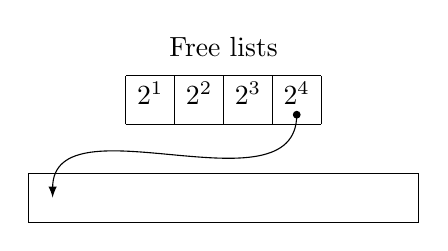
\begin{tikzpicture}[scale=0.62]
            % Boxes
            \draw[step=1] (2,2) grid (6,3);
            \draw (0,0) rectangle (8, 1);
            
            % Labels
            \node[above] at (4, 3.2) {Free lists}; 
            \node[above] at (2.5, 2.2) {$2^1$}; 
            \node[above] at (3.5, 2.2) {$2^2$}; 
            \node[above] at (4.5, 2.2) {$2^3$}; 
            \node[above] at (5.5, 2.2) {$2^4$}; 
            
            % Arrows
            \node[circle,fill,inner sep=1pt] at (5.5, 2.2) {};
            \draw[-latex] (5.5, 2.2) to[out=270, in=90] (0.5, 0.5);
        \end{tikzpicture}
        \caption{\footnotesize Initial memory block}
    \end{subfigure}%
    \begin{subfigure}{.5\textwidth}
        \centering
        \begin{tikzpicture}[scale=0.62]
            % Fills
            \draw[fill=grey] (7,0) rectangle (8,1);
            
            % Boxes
            \draw[step=1] (2,2) grid (6,3);
            \draw (0,0) rectangle (8, 1);
            
            % Labels
            \node[above] at (4, 3.2) {Free lists}; 
            \node[above] at (2.5, 2.2) {$2^1$}; 
            \node[above] at (3.5, 2.2) {$2^2$}; 
            \node[above] at (4.5, 2.2) {$2^3$}; 
            \node[above] at (5.5, 2.2) {$2^4$}; 
            
            % Lines
            \draw (4,0) -- (4, 1);
            \draw (6,0) -- (6, 1);
            \draw (7,0) -- (7, 1);
            
            % Arrows
            \node[circle,fill,inner sep=1pt] at (4.5, 2.2) {};
            \draw[-latex] (4.5, 2.2) to[out=270, in=90] (0.5, 0.5);
            
            \node[circle,fill,inner sep=1pt] at (3.5, 2.2) {};
            \draw[-latex] (3.5, 2.2) to[out=270, in=90] (4.5, 0.5);
            
            \node[circle,fill,inner sep=1pt] at (2.5, 2.2) {};
            \draw[-latex] (2.5, 2.2) to[out=270, in=90] (6.5, 0.5);
        \end{tikzpicture}
        \caption{\footnotesize Allocate an object of size $2^1$}
    \end{subfigure}%
    \vskip 1em
    \begin{subfigure}{.5\textwidth}
        \centering
        \begin{tikzpicture}[scale=0.62]
            % Fills
            \draw[fill=grey] (7,0) rectangle (8,1);
            \draw[fill=grey] (0,0) rectangle (4,1);
            
            % Boxes
            \draw[step=1] (2,2) grid (6,3);
            \draw (0,0) rectangle (8, 1);
            
            % Labels
            \node[above] at (4, 3.2) {Free lists}; 
            \node[above] at (2.5, 2.2) {$2^1$}; 
            \node[above] at (3.5, 2.2) {$2^2$}; 
            \node[above] at (4.5, 2.2) {$2^3$}; 
            \node[above] at (5.5, 2.2) {$2^4$}; 
            
            % Lines
            \draw (4,0) -- (4, 1);
            \draw (6,0) -- (6, 1);
            \draw (7,0) -- (7, 1);
            
            % Arrows
            \node[circle,fill,inner sep=1pt] at (3.5, 2.2) {};
            \draw[-latex] (3.5, 2.2) to[out=270, in=90] (4.5, 0.5);
            
            \node[circle,fill,inner sep=1pt] at (2.5, 2.2) {};
            \draw[-latex] (2.5, 2.2) to[out=270, in=90] (6.5, 0.5);
        \end{tikzpicture}
        \caption{\footnotesize Allocate an object of size $2^3$}
    \end{subfigure}%
    \begin{subfigure}{.5\textwidth}
        \centering
        \begin{tikzpicture}[scale=0.62]
            % Fills
            \draw[fill=grey] (7,0) rectangle (8,1);
            \draw[fill=grey] (0,0) rectangle (4,1);
            \draw[fill=grey] (4,0) rectangle (6,1);
            
            % Boxes
            \draw[step=1] (2,2) grid (6,3);
            \draw (0,0) rectangle (8, 1);
            
            % Labels
            \node[above] at (4, 3.2) {Free lists}; 
            \node[above] at (2.5, 2.2) {$2^1$}; 
            \node[above] at (3.5, 2.2) {$2^2$}; 
            \node[above] at (4.5, 2.2) {$2^3$}; 
            \node[above] at (5.5, 2.2) {$2^4$}; 
            
            % Lines
            \draw (4,0) -- (4, 1);
            \draw (6,0) -- (6, 1);
            \draw (7,0) -- (7, 1);
            
            % Arrows
            \node[circle,fill,inner sep=1pt] at (2.5, 2.2) {};
            \draw[-latex] (2.5, 2.2) to[out=270, in=90] (6.5, 0.5);
        \end{tikzpicture}
        \caption{\footnotesize Allocate an object of size $2^2$}
    \end{subfigure}%
    \vskip 1em
    \begin{subfigure}{.5\textwidth}
        \centering
        \begin{tikzpicture}[scale=0.62]
            % Fills
            \draw[fill=grey] (0,0) rectangle (6,1);
            
            % Boxes
            \draw[step=1] (2,2) grid (6,3);
            \draw (0,0) rectangle (8, 1);
            
            % Labels
            \node[above] at (4, 3.2) {Free lists}; 
            \node[above] at (2.5, 2.2) {$2^1$}; 
            \node[above] at (3.5, 2.2) {$2^2$}; 
            \node[above] at (4.5, 2.2) {$2^3$}; 
            \node[above] at (5.5, 2.2) {$2^4$}; 
            
            % Lines
            \draw (4,0) -- (4, 1);
            \draw (6,0) -- (6, 1);
            \draw (7,0) -- (7, 1);
            
            % Arrows            
            \node[circle,fill,inner sep=1pt] at (2.5, 2.2) {};
            \draw[-latex] (2.5, 2.2) to[out=270, in=90] (7.25, 0.5);

            \node[circle,fill,inner sep=1pt] at (7.75, .5) {};
            \draw[-latex] (7.75, .5) to[out=-135, in=-45] (6.5, .5);
        \end{tikzpicture}
        \caption{\footnotesize Deallocate the object of size $2^1$}
    \end{subfigure}%
    \begin{subfigure}{.5\textwidth}
        \centering
        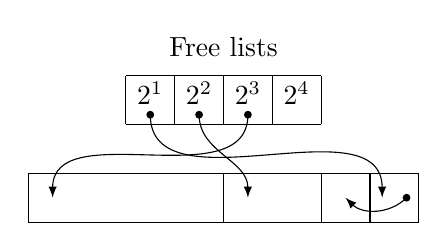
\begin{tikzpicture}[scale=0.62]           
            % Boxes
            \draw[step=1] (2,2) grid (6,3);
            \draw (0,0) rectangle (8, 1);
            
            % Labels
            \node[above] at (4, 3.2) {Free lists}; 
            \node[above] at (2.5, 2.2) {$2^1$}; 
            \node[above] at (3.5, 2.2) {$2^2$}; 
            \node[above] at (4.5, 2.2) {$2^3$}; 
            \node[above] at (5.5, 2.2) {$2^4$}; 
            
            % Lines
            \draw (4,0) -- (4, 1);
            \draw (6,0) -- (6, 1);
            \draw (7,0) -- (7, 1);
            
            % Arrows            
            \node[circle,fill,inner sep=1pt] at (2.5, 2.2) {};
            \draw[-latex] (2.5, 2.2) to[out=270, in=90] (7.25, 0.5);

            \node[circle,fill,inner sep=1pt] at (7.75, .5) {};
            \draw[-latex] (7.75, .5) to[out=-135, in=-45] (6.5, .5);

            \node[circle,fill,inner sep=1pt] at (3.5, 2.2) {};
            \draw[-latex] (3.5, 2.2) to[out=270, in=90] (4.5, 0.5);

            \node[circle,fill,inner sep=1pt] at (4.5, 2.2) {};
            \draw[-latex] (4.5, 2.2) to[out=270, in=90] (0.5, 0.5);
        \end{tikzpicture}
        \caption{\footnotesize Deallocate the object of size $2^3$, then the object of $2^2$}
    \end{subfigure}%
    \caption{Non-opposite deallocation results in a different free list after termination}
    \label{fig:deallocation-order-free-list}
\end{figure}

Figure~\ref{fig:deallocation-order-free-list} shows how alternative deallocation orders results in different free lists, compared to the original given to some function. However, as discussed in section~\ref{sec:memory-garbage}, we can consider every collection of Buddy Memory free lists equivalent, as a later computation can take another set of free lists and still execute its function, as long as the free lists have the required blocks available.

\newpage
\section{Object Allocation and Deallocation}
\label{sec:object-allocation-deallocation}
Now that we have the main allocation mechanism in place and a method of accessing it through a label and a \inst{swapbr} instruction, we can continue translating the \textbf{malloc} procedure entry point from listing~\ref{lst:buddy-memory} on page~\pageref{lst:buddy-memory}.

\begin{figure}[ht!]
    \centering
    \begin{subfigure}{.4\textwidth}
        \lstinputlisting[language=janus, style=basic, frame=none]{buddy-memory-malloc.ja}  
    \end{subfigure}%
    \begin{subfigure}{.5\textwidth}
        \centering
        \resizebox{\linewidth}{!}{
        \begin{minipage}{\linewidth}
            \begin{alignat*}{6}
                &\textbf{(1)}\quad&&l_{malloc\_top}\ \texttt{:}\quad &&\inst{bra}\quad && l_{malloc\_bot}\quad && \quad&& \text{; Receive jump}\\
                &\textbf{(2)}\quad&&l_{malloc}\ \texttt{:}\quad &&\inst{swapbr}\quad &&r_o && && \text{; Entry and exit point}\\
                &\textbf{(3)}\quad&& &&\inst{neg} &&r_o && && \text{; Negate return offset}\\
                &\textbf{(4)}\quad&& &&\inst{addi} &&c_{size} && 2\quad && \text{; Init $c_{size}$}\\
                &\textbf{(5)}\quad&& &&\inst{xor} &&r_{counter} && r_0 && \text{; Init counter}\\
                &\textbf{(6)}\quad&& &&\cdots && && && \text{; Pop $r_p$ and $object_{size}$ from stack}\\
                &\textbf{(7)}\quad&& &&\inst{push} &&r_{0} && && \text{; Push $r_o$}\\
                &\textbf{(8)}\quad&& &&\inst{bra} &&l_{malloc1} && && \text{; call \textbf{malloc1()}}\\
                &\textbf{(9)}\quad&& &&\inst{pop} &&r_{0} && && \text{; Inverse of \textbf{(7)}}\\
                &\textbf{(10)}\quad&& &&\cdots &&r_{0} && && \text{; Inverse of \textbf{(6)}}\\
                &\textbf{(11)}\quad&& &&\inst{xor} &&r_{counter} && r_0 && \text{; Inverse of \textbf{(5)}}\\
                &\textbf{(12)}\quad&& &&\inst{subi} &&c_{size} && 2 && \text{; Inverse of \textbf{(4)}}\\
                &\textbf{(13)}\quad&&l_{malloc\_bot}\ \texttt{:}\quad &&\inst{bra} &&l_{malloc\_top} && && \text{; Jump}\\
            \end{alignat*}
        \end{minipage}
        }
    \end{subfigure}
    \caption{\textsc{Pisa} translation of the \textbf{malloc} procedure entry point of Buddy Memory algorithm}
    \label{fig:pisa-buddy-malloc-entry}
\end{figure}

Figure~\ref{fig:pisa-buddy-malloc-entry} shows the translated \textbf{malloc} procedure. In addition to the original procedure, we also push the current return offset register value to the stack before we branch to the \textbf{malloc1} implementation, to ensure we have a zero-cleared register before starting the allocation process. The translated procedure assumes that the pointer to the object we are allocating and its size are on top of the stack before entering the block. This translated procedure serves as the entry point for the allocation subroutine as it is also only generated once. Each \textbf{new} and \textbf{delete} statement branches to the $l_{malloc}$ label to begin an allocation or a deallocation.  

\begin{figure}[H]
    \centering
    \begin{subfigure}[t]{0.495\linewidth}
        \vskip 0pt
        \centering
        \begin{equation*} 
            \textbf{new}\ c\ x
        \end{equation*}
        \resizebox{.9\linewidth}{!}{
            \begin{minipage}{\linewidth}
                \begin{alignat*}{5}
                    &\textbf{(1)}\quad&&\cdots \quad &&\quad && \quad &&\text{; Push registers }\\
                    &\textbf{(2)}\quad&&\cdots\quad &&\quad && &&\text{; Code for $r_t \leftarrow x_{size}$}\\
                    &\textbf{(3)}\quad&&\inst{push}\quad && r_t \quad && &&\text{; Push $r_t$}\\
                    &\textbf{(4)}\quad&&\inst{push}\quad && r_p \quad && &&\text{; Push $r_p$}\\
                    &\textbf{(5)}\quad&&\inst{bra}\quad && l_{malloc} \quad && &&\text{; Allocate}\\
                    &\textbf{(6)}\quad&&\inst{pop}\quad && r_p \quad && &&\text{; Inverse of \textbf{(4)}}\\
                    &\textbf{(7)}\quad&&\inst{pop}\quad && r_t \quad && &&\text{; Inverse of \textbf{(3)}}\\
                    &\textbf{(8)}\quad&&\cdots\quad && \quad && &&\text{; Inverse of \textbf{(2)}}\\
                    &\textbf{(9)}\quad&&\cdots\quad && \quad && &&\text{; Inverse of \textbf{(1)}}\\
                    &\textbf{(10)}\quad&&\cdots\quad &&\quad && &&\text{; Code for $r_v \leftarrow \llbracket addr(x) \rrbracket$}\\
                    &\textbf{(11)}\quad&&\inst{xori}\quad && r_t\quad && label_{vt} &&\text{; Store address of vtable in $r_t$}\\
                    &\textbf{(12)}\quad&&\inst{exch}\quad && r_t\quad && r_p\quad &&\text{; Store vtable in new object}\\
                    &\textbf{(13)}\quad&&\inst{addi}\quad && r_p\quad && offset_{ref}\quad &&\text{; Index to ref count pos}\\
                    &\textbf{(14)}\quad&&\inst{xori}\quad && r_t\quad && 1 &&\text{; Init ref count}\\
                    &\textbf{(15)}\quad&&\inst{exch}\quad && r_t\quad && r_p\quad &&\text{; Store ref count}\\
                    &\textbf{(16)}\quad&&\inst{subi}\quad && r_p\quad && offset_{ref}\quad &&\text{; Inverse of \textbf{(13)}}\\
                    &\textbf{(17)}\quad&&\inst{exch}\quad && r_p\quad && r_v\quad &&\text{; Store address in variable}\\
                    &\textbf{(18)}\quad&&\cdots\quad &&\quad && &&\text{; Inverse of \textbf{(10)}}\\
                \end{alignat*}
            \end{minipage}
        }
    \end{subfigure}
    \begin{subfigure}[t]{0.495\linewidth}
        \vskip 0pt
        \centering
        \begin{equation*}
            \textbf{delete}\ c\ x
        \end{equation*}
        \resizebox{.9\linewidth}{!}{
            \begin{minipage}{\linewidth}
                \begin{alignat*}{5}
                    &\textbf{(1)}\quad&&\cdots\quad &&\quad && &&\text{; Code for $r_p \leftarrow \llbracket addr(x) \rrbracket$}\\
                    &\textbf{(2)}\quad&&\inst{exch}\quad && r_t\quad && r_p\quad &&\text{; extract vtable from object}\\
                    &\textbf{(3)}\quad&&\inst{xori}\quad && r_t\quad && label_{vt} &&\text{; clear address of vtable in $r_t$}\\
                    &\textbf{(4)}\quad&&\inst{addi}\quad && r_p\quad && offset_{ref}\quad &&\text{; Index to ref count pos}\\
                    &\textbf{(5)}\quad&&\inst{exch}\quad && r_t\quad && r_p\quad &&\text{; Extract ref count}\\
                    &\textbf{(6)}\quad&&\inst{xori}\quad && r_t\quad && 1 &&\text{; Clear ref count}\\
                    &\textbf{(7)}\quad&&\inst{subi}\quad && r_p\quad && offset_{ref}\quad &&\text{; Inverse of \textbf{(4)}}\\
                    &\textbf{(8)}\quad&&\cdots \quad &&\quad && \quad &&\text{; Push registers except $r_p$, $r_t$ }\\
                    &\textbf{(9)}\quad&&\cdots\quad &&\quad && &&\text{; Code for $r_t \leftarrow x_{size}$}\\
                    &\textbf{(10)}\quad&&\inst{push}\quad && r_t \quad && &&\text{; Push $r_t$}\\
                    &\textbf{(11)}\quad&&\inst{push}\quad && r_p \quad && &&\text{; Push $r_p$}\\
                    &\textbf{(12)}\quad&&\inst{rbra}\quad && l_{malloc} \quad && &&\text{; Deallocate}\\
                    &\textbf{(13)}\quad&&\inst{pop}\quad && r_p \quad && &&\text{; Inverse of \textbf{(11)}}\\
                    &\textbf{(14)}\quad&&\inst{pop}\quad && r_t \quad && &&\text{; Inverse of \textbf{(10)}}\\
                    &\textbf{(15)}\quad&&\cdots\quad &&\quad && &&\text{; Inverse of \textbf{(9)}}\\
                    &\textbf{(16)}\quad&&\cdots\quad && \quad && &&\text{; Inverse of \textbf{(8)}}\\
                    &\textbf{(17)}\quad&&\cdots\quad && \quad && &&\text{; Inverse of \textbf{(1)}}\\
                \end{alignat*}
            \end{minipage}
        }
    \end{subfigure}
    \caption{PISA translation of heap allocation and deallocation for objects}
    \label{fig:pisa-allocation-deallocation}
\end{figure}
\clearpage

Figure~\ref{fig:pisa-allocation-deallocation} shows how each \textbf{new} and \textbf{delete} statement for objects are translated during compilation. They are simply inverse of each other. For allocation, the object pointer and its size are pushed to the stack and then a jump to the malloc entry point is executed. After allocation, the virtual table and reference count are stored in the first two words of the allocated memory. Note how deallocation jumps and flips the direction of execution using the \inst{rbra} instruction, which then runs the allocation process in reverse. In the figure $x_{size}$ denotes the computed size of objects with class $c$, plus two, to account for the virtual table pointer and reference count space, rounded up to nearest power-of-two.

\begin{figure}[ht]
    \centering
    \begin{equation*}
        \textbf{construct}\ c\ x\quad s\quad\textbf{destruct}\ x
    \end{equation*}
    \resizebox{.8\linewidth}{!}{
    \begin{minipage}{\linewidth}
    \begin{alignat*}{6}
    &\textbf{(1)}\quad&&\inst{xor}\quad &&r_x\quad &&r_{sp}\qquad &&\text{; Store address of new object $x$ in $r_x$}\\
    &\textbf{(2)}\quad&&\inst{push}\quad &&r_x\quad && &&\text{; Push $r_x$ to the stack}\\
    &\textbf{(3)}\quad&&\cdots\cdots && && &&\text{; Code for \textbf{new} $c$ $x$}\\
    &\textbf{(4)}\quad&&\cdots\cdots && && &&\text{; Code for statement $s$}\\
    &\textbf{(5)}\quad&&\cdots\cdots && && &&\text{; Code for \textbf{delete} $c$ $x$}\\
    &\textbf{(6)}\quad&&\inst{pop}\quad &&r_x\quad && &&\text{; Pop $r_x$ from the stack}\\
    &\textbf{(7)}\quad&&\inst{xor}\quad &&r_x\quad &&r_{sp}\qquad &&\text{; Clear $r_x$}
    \end{alignat*}
    \end{minipage}
    }
    \caption{PISA translation of a \rooplpp object block}
    \label{fig:pisa-object-block}
\end{figure}

Figure~\ref{fig:pisa-object-block} shows the updated translation technique for object blocks. In \textsc{Roopl}, the object blocks allocated their objects on the stack, but in \rooplpp, we can now allocate them on the heap. to facilitate this, we simply execute the exact same instructions as in \textbf{new} and \textbf{delete} statements, with body statement execution code in between. As described in section~\ref{sec:local-blocks}, the \textbf{construct}/\textbf{desctruct} block can be considered syntactic sugar, and its usage in a real world example would probably be limited.


\section{Referencing}
\label{sec:referencing-compilation}
As mentioned, one of the main strengths of \rooplpp in terms of increased expressiveness is allowance of multiple references to objects and arrays. When an object or array is constructed we allocate enough space to hold an additional \textit{reference counter} which is initialized to $1$. For each reference copied using the \textbf{copy}-statement, we incrementally increase the reference counter by one. When we \textbf{uncopy} a reference, the reference counter is decreased by one. The object or array cannot be deconstructed until its reference counter has been returned to $1$ as we would have a reference pointer to cleared memory in the heap. Such references are known as dangling pointers.

Figure~\ref{fig:ref-counting-object-layout} shows the object layout of \rooplpp objects with the added space for the reference counting from the original \textsc{Roopl} model in figure~\ref{fig:roopl-object-layout} on page~\pageref{fig:roopl-object-layout}.
\newpage

\begin{figure}[ht!]
    \centering
    \begin{subfigure}[t]{.32\textwidth}
        \vspace{0pt}
        \vskip 0pt
        \centering
        \begin{tikzpicture}
            \draw[dashed] (0, 1.5) -- (0, 2);
            \draw[dashed] (3, 1.5) -- (3, 2);
            \filldraw[fill = grey, draw = black] (0, 1) rectangle (3, 1.5) node[midway] {addr(vtable)};
            \filldraw[fill = darkgrey, draw = black] (0, .5) rectangle (3, 1) node[midway] {reference count};
            \filldraw[fill = grey, draw = black] (0, 0) rectangle (3, .5) node[midway] {x};
            \filldraw[fill = darkgrey, draw = black] (0, -.5) rectangle (3, 0) node[midway] {y};
            \draw[dashed] (0, -.5) -- (0, -1);
            \draw[dashed] (3, -.5) -- (3, -1);
    
            \node at (-.3, 1.25) {\texttt{+}$0$};
            \node at (-.3, .75) {\texttt{+}$1$};
            \node at (-.3, .25) {\texttt{+}$2$};
            \node at (-.3, -.25) {\texttt{+}$3$};
            \draw[->] (3.5, 1.25) -- (3.1, 1.25);
            \node[rotate = 270] at (3.7, 1.25) {$r_{shape}$};
            
            \node at (1.5, 2.5) {\textbf{Shape}};
        \end{tikzpicture}
    \end{subfigure}
    \begin{subfigure}[t]{.32\textwidth}
        \vspace{0pt}
        \vskip 0pt
        \centering
        \begin{tikzpicture}
            \draw[dashed] (0, 1.5) -- (0, 2);
            \draw[dashed] (3, 1.5) -- (3, 2);
            \filldraw[fill = grey, draw = black] (0, 1) rectangle (3, 1.5) node[midway] {addr(vtable)};
            \filldraw[fill = darkgrey, draw = black] (0, .5) rectangle (3, 1) node[midway] {reference count};
            \filldraw[fill = grey, draw = black] (0, 0) rectangle (3, .5) node[midway] {x};
            \filldraw[fill = darkgrey, draw = black] (0, -.5) rectangle (3, 0) node[midway] {y};
            \filldraw[fill = grey, draw = black] (0, -1) rectangle (3, -.5) node[midway] {radius};
            \draw[dashed] (0, -1) -- (0, -1.5);
            \draw[dashed] (3, -1) -- (3, -1.5);
    
            \node at (-.3, 1.25) {\texttt{+}$0$};
            \node at (-.3, .75) {\texttt{+}$1$};
            \node at (-.3, .25) {\texttt{+}$2$};
            \node at (-.3, -.25) {\texttt{+}$3$};
            \node at (-.3, -.75) {\texttt{+}$4$};
            \draw[->] (3.5, 1.25) -- (3.1, 1.25);
            \node[rotate = 270] at (3.7, 1.25) {$r_{circ}$};
            
            \node at (1.5, 2.5) {\textbf{Circle}};
        \end{tikzpicture}
    \end{subfigure}
    \begin{subfigure}[t]{.32\textwidth}
        \vspace{0pt}
        \vskip 0pt
        \centering
        \begin{tikzpicture}
            \draw[dashed] (0, 1.5) -- (0, 2);
            \draw[dashed] (3, 1.5) -- (3, 2);
            \filldraw[fill = grey, draw = black] (0, 1) rectangle (3, 1.5) node[midway] {addr(vtable)};
            \filldraw[fill = darkgrey, draw = black] (0, .5) rectangle (3, 1) node[midway] {reference count};
            \filldraw[fill = grey, draw = black] (0, 0) rectangle (3, .5) node[midway] {x};
            \filldraw[fill = darkgrey, draw = black] (0, -.5) rectangle (3, 0) node[midway] {y};
            \filldraw[fill = grey, draw = black] (0, -1) rectangle (3, -.5) node[midway] {a};
            \filldraw[fill = darkgrey, draw = black] (0, -1.5) rectangle (3, -1) node[midway] {b};
            \draw[dashed] (0, -1.5) -- (0, -2);
            \draw[dashed] (3, -1.5) -- (3, -2);
    
            \node at (-.3, 1.25) {\texttt{+}$0$};
            \node at (-.3, .75) {\texttt{+}$1$};
            \node at (-.3, .25) {\texttt{+}$2$};
            \node at (-.3, -.25) {\texttt{+}$3$};
            \node at (-.3, -.75) {\texttt{+}$4$};
            \node at (-.3, -1.25) {\texttt{+}$5$};
            \draw[->] (3.5, 1.25) -- (3.1, 1.25);
            \node[rotate = 270] at (3.7, 1.25) {$r_{rect}$};
            
            \node at (1.5, 2.5) {\textbf{Rectangle}};
        \end{tikzpicture}
    \end{subfigure}
    \caption[Illustration of object memory layout]{Illustration of prefixing in the memory layout of three \rooplpp objects}
    \label{fig:ref-counting-object-layout}
\end{figure}

Figure~\ref{fig:pisa-referencing} shows the translated \textsc{Pisa} code for the \textbf{copy} and \textbf{uncopy} statements. As shown, they are both very simple and each others inverse. For copying, the address of the passed variable $x$ is simply copied into the zero-cleared value of $x'$ and the reference count incremented by one. For deletion, the address is cleared and the reference count decremented. Copying and clearing is done through the \inst{xor} instruction. These translations features no error handling, but a solution is discussed in section~\ref{sec:error-handling}.

\begin{figure}[ht]
    \centering
    
    \begin{subfigure}[t]{0.495\linewidth}
    \vskip 0pt
    \centering
    \begin{equation*} 
        \textbf{copy}\ c\ x\ x'
    \end{equation*}
    
    \resizebox{.8\linewidth}{!}{
        \begin{minipage}{1.025\linewidth}
            \begin{alignat*}{5}
                &\textbf{(1)}\quad&&\dots\quad && && &&\text{; Code for $r_{p}\ \leftarrow\ addr(x)$}\\
                &\textbf{(2)}\quad&&\dots\quad && && &&\text{; Code for $r_{cp}\ \leftarrow\ value(x')$}\\
                &\textbf{(3)}\quad&&\inst{xor}\quad &&r_{cp}\quad && r_p \quad &&\text{; Copy address of $x$ into $x'$}\\
                &\textbf{(4)}\quad&&\inst{addi}\quad &&r_{p}\quad && offset_{ref} &&\text{; Index to reference count address}\\
                &\textbf{(5)}\quad&&\inst{exch}\quad &&r_{t}\quad && r_p &&\text{; Extract reference count}\\
                &\textbf{(6)}\quad&&\inst{addi}\quad &&r_{t}\quad && 1 &&\text{; Increment reference count}\\
                &\textbf{(7)}\quad&&\inst{exch}\quad &&r_{t}\quad && r_p &&\text{; Store updated reference count}\\
                &\textbf{(8)}\quad&&\inst{subi}\quad &&r_{p}\quad && offset_{ref} &&\text{; Inverse of \textbf{(3)}}\\
                &\textbf{(9)}\quad&&\dots\quad && && &&\text{; Inverse of \textbf{(2)}}\\
                &\textbf{(10)}\quad&&\dots\quad && && &&\text{; Inverse of \textbf{(1)}}
            \end{alignat*}
        \end{minipage}
    }
    \end{subfigure}
    \begin{subfigure}[t]{0.495\linewidth}
    \vskip 0pt
    \centering
    \begin{equation*}
        \textbf{uncopy}\ c\ x\ x'
    \end{equation*}
    
    \resizebox{.8\linewidth}{!}{
        \begin{minipage}{1.025\linewidth}
            \begin{alignat*}{5}
                &\textbf{(1)}\quad&&\dots\quad && && &&\text{; Code for $r_{p}\ \leftarrow\ addr(x)$}\\
                &\textbf{(2)}\quad&&\dots\quad && && &&\text{; Code for $r_{cp}\ \leftarrow\ value(x')$}\\
                &\textbf{(3)}\quad&&\inst{xor}\quad &&r_{cp}\quad && r_p \quad &&\text{; Clear address of $x$ from $x'$}\\
                &\textbf{(4)}\quad&&\inst{addi}\quad &&r_{p}\quad && offset_{ref} &&\text{; Index to reference count address}\\
                &\textbf{(5)}\quad&&\inst{exch}\quad &&r_{t}\quad && r_p &&\text{; Extract reference count}\\
                &\textbf{(6)}\quad&&\inst{subi}\quad &&r_{t}\quad && 1 &&\text{; Decrement reference count}\\
                &\textbf{(7)}\quad&&\inst{exch}\quad &&r_{t}\quad && r_p &&\text{; Store updated reference count}\\
                &\textbf{(8)}\quad&&\inst{subi}\quad &&r_{p}\quad && offset_{ref} &&\text{; Inverse of \textbf{(3)}}\\
                &\textbf{(9)}\quad&&\dots\quad && && &&\text{; Inverse of \textbf{(2)}}\\
                &\textbf{(10)}\quad&&\dots\quad && && &&\text{; Inverse of \textbf{(1)}}
            \end{alignat*}
        \end{minipage}
    }
    \end{subfigure}
    
    \caption{\textsc{Pisa} translation of the reference copying and deletion statements}
    \label{fig:pisa-referencing}
\end{figure}

\section{Arrays}
\label{sec:arrays}
The fixed-sized arrays in \rooplpp are also heap allocated to allow dynamic lifetime. The array memory layout is presented in figure~\ref{fig:array-layout}. As shown, the arrays feature two additional fields to store the size of the array and the reference count. Additionally, integer arrays store their values directly in the array, while object arrays are a simple pointer stores.

As the size of a \rooplpp array is determined by a passed expression evaluation, it is unknown at compile time. This also means that out-of-bounds checking cannot be conducted during compilation. A possible solution for this is presented in section~\ref{sec:error-handling}.  

\begin{figure}[ht]
    \centering
    \begin{subfigure}[ht]{.32\textwidth}
        \vskip 0pt
        \centering
        \begin{tikzpicture}
            \draw[dashed] (0, 2) -- (0, 2.5);
            \draw[dashed] (3, 2) -- (3, 2.5);
            \filldraw[fill = darkgrey, draw = black] (0, 1.5) rectangle (3, 2) node[midway] {$\llbracket e \rrbracket$};
            \filldraw[fill = grey, draw = black] (0, 1) rectangle (3, 1.5) node[midway] {reference count};
            \filldraw[fill = darkgrey, draw = black] (0, .5) rectangle (3, 1) node[midway] {$x[0]$ (value)};
            \filldraw[fill = grey, draw = black] (0, 0) rectangle (3, .5) node[midway] {$x[1]$ (value)};
            \draw[dashed] (0, 0) -- (0, -.5);
            \node at (1.5, -.25) {$\dots$};
            \draw[dashed] (3, 0) -- (3, -.5);
            \filldraw[fill = grey, draw = black] (0, -.5) rectangle (3, -1) node[midway] {$x[n]$ (value)};
            \draw[dashed] (0, -1) -- (0, -1.5);
            \draw[dashed] (3, -1) -- (3, -1.5);
    
            \node at (-.3, 1.75) {\texttt{+}$0$};
            \node at (-.3, 1.25) {\texttt{+}$1$};
            \node at (-.3, .75) {\texttt{+}$2$};
            \node at (-.3, .25) {\texttt{+}$3$};
            \node at (-.6, -.75) {\texttt{+}$n+1$};
            \draw[->] (3.5, 1.75) -- (3.1, 1.75);
            \node[rotate = 270] at (3.7, 1.75) {$r_{x}$};
            
            \node at (1.5, 3) {\textbf{int}[$e$] $x$};
        \end{tikzpicture}
    \end{subfigure}
    \begin{subfigure}[ht]{.32\textwidth}
        \vskip 0pt
        \centering
        \begin{tikzpicture}
            \draw[dashed] (0, 2) -- (0, 2.5);
            \draw[dashed] (3, 2) -- (3, 2.5);
            \filldraw[fill = darkgrey, draw = black] (0, 1.5) rectangle (3, 2) node[midway] {$\llbracket e \rrbracket$};
            \filldraw[fill = grey, draw = black] (0, 1) rectangle (3, 1.5) node[midway] {reference count};
            \filldraw[fill = darkgrey, draw = black] (0, .5) rectangle (3, 1) node[midway] {$y[0]$ (address)};
            \filldraw[fill = grey, draw = black] (0, 0) rectangle (3, .5) node[midway] {$y[1]$ (address)};
            \draw[dashed] (0, 0) -- (0, -.5);
            \node at (1.5, -.25) {$\dots$};
            \draw[dashed] (3, 0) -- (3, -.5);
            \filldraw[fill = grey, draw = black] (0, -.5) rectangle (3, -1) node[midway] {$y[n]$ (address)};
            \draw[dashed] (0, -1) -- (0, -1.5);
            \draw[dashed] (3, -1) -- (3, -1.5);
    
            \node at (-.3, 1.75) {\texttt{+}$0$};
            \node at (-.3, 1.25) {\texttt{+}$1$};
            \node at (-.3, .75) {\texttt{+}$2$};
            \node at (-.3, .25) {\texttt{+}$3$};
            \node at (-.6, -.75) {\texttt{+}$n+1$};
            \draw[->] (3.5, 1.75) -- (3.1, 1.75);
            \node[rotate = 270] at (3.7, 1.75) {$r_{y}$};
            
            \node at (1.5, 3) {\textbf{Shape}[$e$] $y$};
        \end{tikzpicture}
    \end{subfigure}
    \caption{Illustration of prefixing in the memory layout of two \rooplpp arrays}
    \label{fig:array-layout}
\end{figure}
\newpage
\subsection{Construction and Destruction}
\label{subsec:construction-destruction}
As \rooplpp arrays also are heap allocated, the buddy allocation implementation is also used for allocating arrays. The only difference between object and array allocation is that no virtual table is stored in the allocated space while the offsets for the reference counter are shared for both types. Due to this fact, \textbf{copy} and \textbf{uncopy} \textsc{Pisa} blocks generated during compile time are exactly the same for arrays and objects, as shown in the previous section.

\begin{figure}[ht]
    \centering
    \begin{subfigure}[t]{0.495\linewidth}
        \vskip 0pt
        \centering
        \begin{equation*} 
            \textbf{new}\ a[e]\ x
        \end{equation*}
        \resizebox{.9\linewidth}{!}{
            \begin{minipage}{\linewidth}
                \begin{alignat*}{5}
                    &\textbf{(1)}\quad&&\cdots \quad &&\quad && \quad &&\text{; Push registers }\\
                    &\textbf{(2)}\quad&&\cdots\quad &&\quad && &&\text{; Code for $r_t \leftarrow \llbracket e \rrbracket + 2$}\\
                    &\textbf{(3)}\quad&&\inst{push}\quad && r_t \quad && &&\text{; Push $r_t$}\\
                    &\textbf{(4)}\quad&&\inst{push}\quad && r_p \quad && &&\text{; Push $r_p$}\\
                    &\textbf{(5)}\quad&&\inst{bra}\quad && l_{malloc} \quad && &&\text{; Allocate array}\\
                    &\textbf{(6)}\quad&&\inst{pop}\quad && r_p \quad && &&\text{; Inverse of \textbf{(4)}}\\
                    &\textbf{(7)}\quad&&\inst{pop}\quad && r_t \quad && &&\text{; Inverse of \textbf{(3)}}\\
                    &\textbf{(9)}\quad&&\cdots\quad && \quad && &&\text{; Inverse of \textbf{(1)}}\\
                    &\textbf{(10)}\quad&&\cdots\quad &&\quad && &&\text{; Code for $r_v \leftarrow \llbracket addr(x) \rrbracket$}\\
                    &\textbf{(11)}\quad&&\inst{subi}\quad && r_t\quad && 2 &&\text{; $r_t \leftarrow \llbracket e \rrbracket$}\\
                    &\textbf{(12)}\quad&&\inst{exch}\quad && r_t\quad && r_p\quad &&\text{; Store size in new array}\\
                    &\textbf{(13)}\quad&&\inst{addi}\quad && r_p\quad && offset_{ref}\quad &&\text{; Index to ref count pos}\\
                    &\textbf{(14)}\quad&&\inst{xori}\quad && r_t\quad && 1 &&\text{; Init ref count}\\
                    &\textbf{(15)}\quad&&\inst{exch}\quad && r_t\quad && r_p\quad &&\text{; Store ref count}\\
                    &\textbf{(16)}\quad&&\inst{subi}\quad && r_p\quad && offset_{ref}\quad &&\text{; Inverse of \textbf{(13)}}\\
                    &\textbf{(17)}\quad&&\inst{exch}\quad && r_p\quad && r_v\quad &&\text{; Store address in variable}\\
                    &\textbf{(18)}\quad&&\cdots\quad &&\quad && &&\text{; Inverse of \textbf{(10)}}\\
                \end{alignat*}
            \end{minipage}
        }
    \end{subfigure}
    \begin{subfigure}[t]{0.495\linewidth}
        \vskip 0pt
        \centering
        \begin{equation*}
            \textbf{delete}\ a[e]\ x
        \end{equation*}
        \resizebox{.9\linewidth}{!}{
            \begin{minipage}{\linewidth}
                \begin{alignat*}{5}
                    &\textbf{(1)}\quad&&\cdots\quad &&\quad && &&\text{; Code for $r_p \leftarrow \llbracket addr(x) \rrbracket$}\\
                    &\textbf{(2)}\quad&&\cdots\quad && \quad && \quad &&\text{; Code for $r_v \leftarrow \llbracket e \rrbracket$}\\
                    &\textbf{(3)}\quad&&\inst{addi}\quad && r_p\quad && offset_{ref}\quad &&\text{; Index to ref count pos}\\
                    &\textbf{(4)}\quad&&\inst{exch}\quad && r_t\quad && r_p\quad &&\text{; Extract ref count}\\
                    &\textbf{(5)}\quad&&\inst{xori}\quad && r_t\quad && 1 &&\text{; Clear ref count}\\
                    &\textbf{(6)}\quad&&\inst{subi}\quad && r_p\quad && offset_{ref}\quad &&\text{; Inverse of \textbf{(3)}}\\
                    &\textbf{(7)}\quad&&\inst{exch}\quad && r_t\quad && r_p\quad &&\text{; extract size from object}\\
                    &\textbf{(8)}\quad&&\inst{xori}\quad && r_t\quad && r_v &&\text{; clear size in $r_t$}\\
                    &\textbf{(9)}\quad&&\cdots \quad &&\quad && \quad &&\text{; Push registers except $r_p$, $r_v$ }\\
                    &\textbf{(10)}\quad&&\inst{addi}\quad && r_v \quad && 2 &&\text{; Actual size of array}\\
                    &\textbf{(11)}\quad&&\inst{push}\quad && r_v \quad && &&\text{; Push $r_v$}\\
                    &\textbf{(12)}\quad&&\inst{push}\quad && r_p \quad && &&\text{; Push $r_p$}\\
                    &\textbf{(13)}\quad&&\inst{rbra}\quad && l_{malloc} \quad && &&\text{; Deallocate array}\\
                    &\textbf{(14)}\quad&&\inst{pop}\quad && r_p \quad && &&\text{; Inverse of \textbf{(12)}}\\
                    &\textbf{(15)}\quad&&\inst{pop}\quad && r_v \quad && &&\text{; Inverse of \textbf{(11)}}\\
                    &\textbf{(16)}\quad&&\inst{subi}\quad && r_v \quad && 2 &&\text{; Inverse of \textbf{(10)}}\\
                    &\textbf{(17)}\quad&&\cdots\quad &&\quad && &&\text{; Inverse of \textbf{(9)}}\\
                    &\textbf{(18)}\quad&&\cdots\quad && \quad && &&\text{; Inverse of \textbf{(2)}}\\
                    &\textbf{(19)}\quad&&\cdots\quad && \quad && &&\text{; Inverse of \textbf{(1)}}\\
                \end{alignat*}
            \end{minipage}
        }
    \end{subfigure}
    \caption{\textsc{Pisa} translations of array allocation and deallocation statements}
    \label{fig:array-allocation-deallocation}
\end{figure}

Figure~\ref{fig:array-allocation-deallocation} shows the translation schemes used for array allocation and deallocation. As said, these are almost identical to the object allocation and deallocation schemes presented in figure~\ref{fig:pisa-allocation-deallocation} on page~\pageref{fig:pisa-allocation-deallocation}. Classes are analyzed during a compilation phase and their allocation size, the object size + 2 (for virtual table and reference counter) rounded up to nearest power-of-two. The size of arrays cannot be determined during compilation, as that would require evaluating the expression passed to the initialization call, and as such, we add the overhead needed directly in the allocation and deallocation instructions. While the two blocks are code are not exact opposites they are functionally inverse of each other. An extra \inst{xori} instruction on line \textbf{(8)} in the deallocation block has been included to clear the stored array size using the value of the passed expression and further use this size for the inverse \textbf{malloc} subroutine.  

\begin{figure}[ht]
    \centering
        \begin{subfigure}{.75\textwidth}
            \centering
            \begin{tikzpicture}[scale=0.75]
                % Fills
                \draw[fill=grey] (4,0) rectangle (8,1);
                
                % Boxes
                \draw (0,0) rectangle (8, 1);

                % lines
                \draw[dotted] (5, 0) to (5, 1);
                \draw[dotted] (6, 0) to (6, 1);
                \draw[dotted] (7, 0) to (7, 1);
                \draw[dotted] (8, 0) to (8, 1);

                % pointer
                \draw[->] (4.5, 1.5) -- (4.5, 1.1);
                \node[above] at (4.5, 1.5) {\small $c[2]\ x$};

                % labels
                \node[above] at (4.5, 0.15) {\small $2$}; 
                \node[above] at (5.5, 0.15) {\small $1$};
                \node[above] at (6.5, 0.15) {\small \textbf{nil}}; 
                \node[above] at (7.5, 0.15) {\small \textbf{nil}}; 
            \end{tikzpicture}
            \caption{\footnotesize Allocate an array of class $c$ and size $2$ in $x$ by $\textbf{new}\ c[2]\ x$}
        \end{subfigure}%
        \vskip 1em
        \begin{subfigure}[t]{.5\textwidth}
            \vspace{0pt}
            \vskip 0pt
            \centering
            \begin{tikzpicture}[scale=0.75]
                % Fills
                \draw[fill=grey] (4,0) rectangle (8,1);
                \draw[fill=grey] (2,0) rectangle (4,1);
                
                % Boxes
                \draw (0,0) rectangle (8, 1);

                % lines
                \draw[dotted] (5, 0) to (5, 1);
                \draw[dotted] (6, 0) to (6, 1);
                \draw[dotted] (7, 0) to (7, 1);
                \draw[dotted] (8, 0) to (8, 1);

                % pointer
                \draw[->] (4.5, 1.5) -- (4.5, 1.1);
                \node[above] at (4.5, 1.5) {\small $c[2]\ x$};

                % labels
                \node[above] at (3, 0.15) {\small $c$};
                \node[above] at (4.5, 0.15) {\small $2$}; 
                \node[above] at (5.5, 0.15) {\small $1$};
                \node[above] at (7.5, 0.15) {\small \textbf{nil}};                

                % Arrows
                \node[circle,fill,inner sep=1pt] at (6.5, 0.5) {};
                \draw[-latex] (6.5, 0.5) to[out=-90, in=-90] (2.5, 0.5);
                \draw[-latex, white] (7.5, 0.5) to[out=-90, in=-90] (0.5, 0.5);
                \draw (0,0) rectangle (8, 1);
            \end{tikzpicture}
            \caption{\footnotesize Assign first cell with $\textbf{new}\ c\ x[0]$}
        \end{subfigure}%
        \begin{subfigure}[t]{.5\textwidth}
            \vspace{0pt}
            \vskip 0pt
            \centering
            \begin{tikzpicture}[scale=0.75]
                % Fills
                \draw[fill=grey] (4,0) rectangle (8,1);
                \draw[fill=grey] (2,0) rectangle (4,1);
                \draw[fill=grey] (0,0) rectangle (2,1);
                
                % Boxes
                \draw (0,0) rectangle (8, 1);

                % lines
                \draw[dotted] (5, 0) to (5, 1);
                \draw[dotted] (6, 0) to (6, 1);
                \draw[dotted] (7, 0) to (7, 1);
                \draw[dotted] (8, 0) to (8, 1);

                % pointer
                \draw[->] (4.5, 1.5) -- (4.5, 1.1);
                \node[above] at (4.5, 1.5) {\small $c[2]\ x$};

                % labels
                \node[above] at (1, 0.15) {\small $c$};
                \node[above] at (3, 0.15) {\small $c$};
                \node[above] at (4.5, 0.15) {\small $2$}; 
                \node[above] at (5.5, 0.15) {\small $1$};               

                % Arrows
                \node[circle,fill,inner sep=1pt] at (6.5, 0.5) {};
                \draw[-latex] (6.5, 0.5) to[out=-90, in=-90] (2.5, 0.5);

                \node[circle,fill,inner sep=1pt] at (7.5, 0.5) {};
                \draw[-latex] (7.5, 0.5) to[out=-90, in=-90] (0.5, 0.5);
            \end{tikzpicture}
            \caption{\footnotesize Assign next cell with $\textbf{new}\ c\ x[1]$}
        \end{subfigure}%
    \caption{Illustration of array memory storage layout}
    \label{fig:array-memory-storage}
\end{figure}

Figure~\ref{fig:array-memory-storage} shows how object arrays simply contain pointers to allocated objects. For integer arrays, the cell values would stored directly in the allocated array space instead. 

\subsection{Array Element Access}
\label{subsec:array-element-access}
Array elements are simply passed as any other variable to methods or statements. Based on the variable type, compilation of various statements individually determines whether the address or the value of the passed variable should be used for the compiling the statement. For arrays, this is no different. If an integer array element is passed, it is treated just liked a regular integer variable. For an object array element, it is treated just like a regular object variable. 


\section{Error Handling}
\label{sec:error-handling}
While a program written in \rooplpp might be syntactically valid and well-typed, this is not a guarantee that it executes successfully. A number of conditions exist, which cannot be determined at compile time, which in turn results in erroneous executed code. \citeauthor{th:roopl} describes the following conditions:

\begin{itemize}
    \item If the entry expression of a conditional is \textbf{true}, then the exit assertion should also be \textbf{true} after executing the then-branch.
    \item If the entry expression of a conditional is \textbf{false}, then the exit assertion should also be \textbf{false} after executing the else-branch.
    \item The entry expression of a loop should initially be \textbf{true}.
    \item If the exit assertion of a loop is \textbf{false}, then the entry expression should also be \textbf{false} after executing the loop-statement.
    \item All instance variables should be zero-cleared within an object block before the object is deallocated.
    \item The value of a local variable should always match the value of the delocal-expression after the block statement has executed~\cite{th:roopl}.
\end{itemize}

The extensions made to \textsc{Roopl} in \rooplpp brings forth a number of additional conditions:

\begin{itemize}
    \item All fields of an object instance should be zero-cleared before the object is deallocated using the \textbf{delete} statement.
    \item All cells of an instance should be zero-cleared before the array is deallocated using the \textbf{delete} statement.
    \item Local object blocks should have their fields zero-cleared after the execution of the block statement.
    \item Local array blocks should have their cells zero-cleared after the execution of the block statement.
    \item If the value of a local object variable is exchanged during its block statement and the new value is an object reference, this object must have its fields zero-cleared after the execution of the block statement.
    \item If the value of a local array variable is exchanged during its block statement and the new value is an array reference, this array must have its cell zero-cleared after the execution of the block statement.
    \item The variable in the \textbf{new} statement must be zero-cleared beforehand.
    \item The variable in the \textbf{copy} statement must be zero-cleared beforehand.
    \item An object variable must be initialized using \textbf{new} or \textbf{copy} before its methods can be called.
    \item An array variable must be initialized using \textbf{new} or \textbf{copy} before its fields can be accessed.
    \item Array cell indices must be within bounds defined in the expression passed during initialization.
    \item Only one reference to an object or an array must exist when executing the \textbf{delete} statement.
    \item Swapping cell values between a subtype $A$ variable and parent-type $B$ array is only allowed if the value stored in the variable is also $A$ afterwards.
\end{itemize}

It is the programmer's responsibility to meet these conditions. As these conditions, in general, cannot be determined at compile time, undefined program behaviour will occur as the termination will continue silently, resulting in erroneous program state. We can insert run time error checks in the generated instructions such that the program is terminated if one of the conditions does not hold. The run time error checks can be added as dynamic error checks using error routines defined at labels, such as $label_{uninitialized\_object}$ which the program can jump to, if such a condition is unmet. \citeauthor{th:roopl} presented an example for dynamic error checking for local blocks in~\cite{th:roopl}. \textsc{Pisa} and its simulator PendVM is, however, limited and does not support exit codes natively. To fully support dynamic error checking, PendVM could be extended to read from a value from a designated register to supply a more meaningful message for the programmer in the case of a run time exit.
 
\section{Implementation}
\label{sec:implementation}
The \rooplpp compiler (\textsc{Rooplppc}) was implemented using techniques and translation schemes presented in this chapter, expanding upon the work of the original \textsc{Roopl} compiler (\textsc{Rooplc}). The compiler serves as a proof-of-concept and simply performs one-to-one translations of \rooplpp code to \textsc{Pisa} code without any optimizations along the way. The compiler is written in \textsc{Haskell} 7.10 and the translated output was tested on the Pendulum simulator, PendVM~\cite{cr:pendvm}. 

As with the \textsc{Roopl} compiler, the \rooplpp compiler is structured around the same six separate compilation phases.
\begin{enumerate}
    \item \textbf{Parsing} consists of constructing an abstract syntax tree from the input program text using parser combinators from the \textsc{Parsec} library in \textsc{Haskell}.
    \item \textbf{Class Analysis} verifies inheritance cycles, duplicated method names or fields and base classes. In this phase, we also compute the allocation size of each class
    \item \textbf{Scope Analysis} constructs the virtual and symbol tables and maps every identifier to a unique variable or method.
    \item \textbf{Type Checking} verifies that the parsed program is well-typed.
    \item \textbf{Code Generation} translates the abstract syntax tree to blocks of \textsc{Pisa} code in a recursive descent.
    \item \textbf{Macro Expansion} expands macros left by the code generator for i.e. configuration variables, etc.
\end{enumerate}

Compiled \textsc{Roopl} programs have a size increase by a factor of 10 to 15 in terms of the lines of code. For \rooplpp the size increase is much larger, partially due to the increase of static code included in form of the memory manager using the buddy layout described in this chapter and partially because heap allocations are more costly than stack allocations in terms of lines of code.

The \textsc{Roopl} compiler was implemented in $1403$ lines of \textsc{Haskell} and the \rooplpp compiler was extended to $2046$ lines of \textsc{Haskell}.

The entire compiler source code as well as example programs and their compiled versions are provided in the appendices and in the supplied ZIP archive. It is also hosted on Github as open source software under the MIT license at \url{https://github.com/cservenka/ROOPLPPC}.

Building and usage of the compiler is supplied in the README.md file found in the ZIP archive and in appendix~\ref{app:rooplc-source}.

\section{Evaluation}
\label{sec:evaluation}
For evaluating the results of the implemented compiler, it was tested against example code provided throughout this thesis. Tests programs utilizing the linked list, doubly-linked list and binary tree data structures and the RTM implementation are found in appendix~\ref{app:example-output}.

\begin{figure}[ht]
    \centering
    \begin{tabular}{ c | c | c | c}
        \textbf{Program} & \textbf{\rooplpp LOC} & \textbf{\textsc{Pisa} LOC} & \textbf{Number of executed instructions}  \\ \hline 
        Linked List & 61 & 1280 & 18015 \\
        Doubly-Linked List & 66 & 1339 & 21825 \\
        Binary Tree & 86 & 2056 & 6065\\ 
        RTM Simulation & 211 & 6716 & 64922\\ 
      \end{tabular}
    \caption{Lines of code comparison between target and compiled \rooplpp programs}
    \label{fig:lines-of-code}
\end{figure}

The linked list test programs simply instantiates ten cells and links them in their respective lists. The binary tree test program instantiates three nodes and adds them to the tree structure, which afterwards is traversed to determine the sum of the nodes and finally mirroring the tree. The Reversible Turing Machine implementing incrementation of a non-negative $n$-bit binary number by 1 originally described in~\cite{ty:ejanus} has been implemented in \rooplpp and successfully converts its initial tape value in little endian form of $1101$ to $0011$ after termination. It should be noted that these test programs require additional stack space during their lengthy computations and as such has been compiled with twice the length between the stack and heap to allow further stack growth.

As discussed, the compiler is considered proof-of-concept and no noteworthy optimizations has been implemented. However, for the sake of giving the reader an idea of the size blowup of a compiled \rooplpp program, figure~\ref{fig:lines-of-code} details this difference. The lines of translated \textsc{Pisa} instructions includes the $204$ instructions needed for the \textbf{malloc} and \textbf{malloc1} \textsc{Pisa}-equivalent mechanisms. The last row of the table shows how many instructions are execution during simulation using PendVM.


